\chapter{Implementation of Ordinary Kriging}
\label{ch:kriging}

%=============================================================================
\section{Pipeline overview}
\label{sec:kriging-pipeline}
%=============================================================================

Ordinary Kriging is implemented as the geostatistical baseline against which
gradient boosting (Chapter~\ref{ch:gbm}) and Bayesian Neural Fields
(Chapter~\ref{ch:bayesnf}) are evaluated. The pipeline follows the two-stage
decomposition $Z = I \cdot A$ from
Section~\ref{sec:kriging-indicator}: a binary indicator stage produces a
wet/dry classification, and an amount stage predicts precipitation magnitude
on cells classified as wet. The amount stage operates in three steps:
climatological normalisation (Section~\ref{sec:detrending}) removes seasonal
and orographic non-stationarity, Ordinary Kriging is solved on the normalised
values, and a Monte Carlo back-transformation maps the prediction back to
physical millimetres. Cross-validation uses the 5-fold station split shared
with the gradient boosting and BayesNF chapters on 1{,}966 training stations,
with 492 holdout stations reserved for the final test.

\begin{figure}[ht]
    \centering
    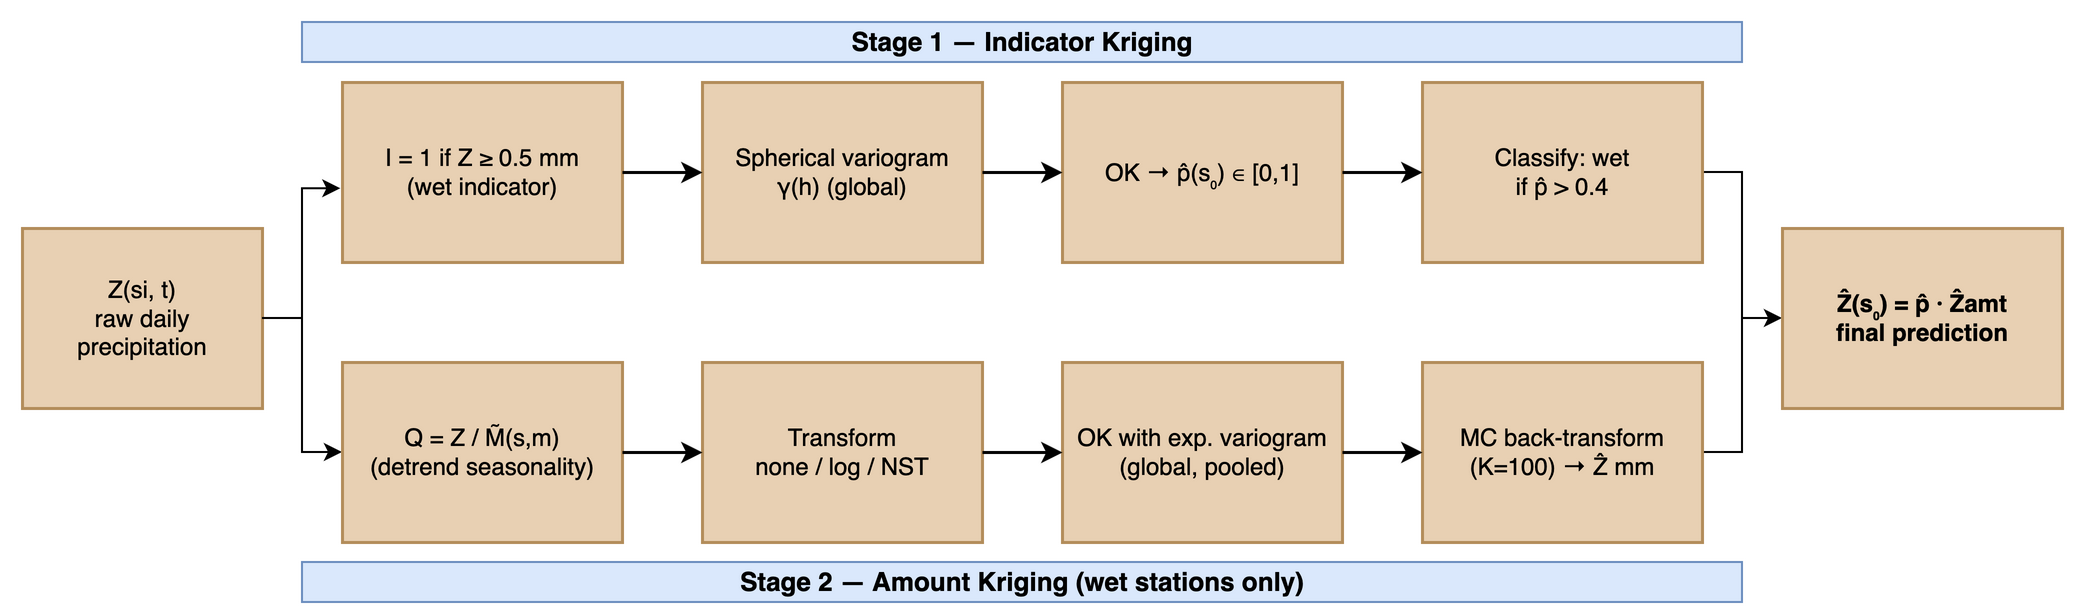
\includegraphics[width=0.95\textwidth]{images/04/two_stage_architecture}
    \caption{Two-stage kriging pipeline. Stage~1 produces a binary
    wet/dry mask via indicator kriging; Stage~2 interpolates the
    climatological ratio at wet cells and back-transforms to physical
    millimetres}
    \label{fig:two-stage-architecture}
\end{figure}

%=============================================================================
\section{Stage~1: indicator kriging}
\label{sec:kriging-indicator-impl}
%=============================================================================

Stage~1 implements the indicator decision of
Equation~\eqref{eq:indicator-decision} using the \texttt{PyKrige} Python
library. Each station observation is converted to a wet-day indicator
$I = \mathbf{1}[Z \geq \tau]$ with threshold $\tau = 0{.}5$~mm — the
standard E-OBS value, chosen above the typical $0{.}1$--$0{.}2$~mm gauge
measurement accuracy \cite{haylock2008european}.
Following Hofstra et al.~\cite{hofstra2008comparison}, a \textbf{spherical}
variogram is used for the indicator field
(Figure~\ref{fig:indicator-variogram}). The model is fitted globally by
pooling empirical indicator semi-variance across all wet days of the
1961--2023 record, excluding days on which all stations are wet or all are
dry (the indicator has zero variance in those cases). Ordinary Kriging on
the binary inputs produces, at every grid cell, the wet-day probability
$\hat{p}(\mathbf{s}_0)$. The decision threshold $p^{\star} = 0{.}4$
\cite{hofstra2008comparison} converts this probability into a binary
classification: cells with $\hat{p} > 0{.}4$ are passed to Stage~2, the
remaining cells are set to zero precipitation.

\begin{figure}[H]
    \centering
    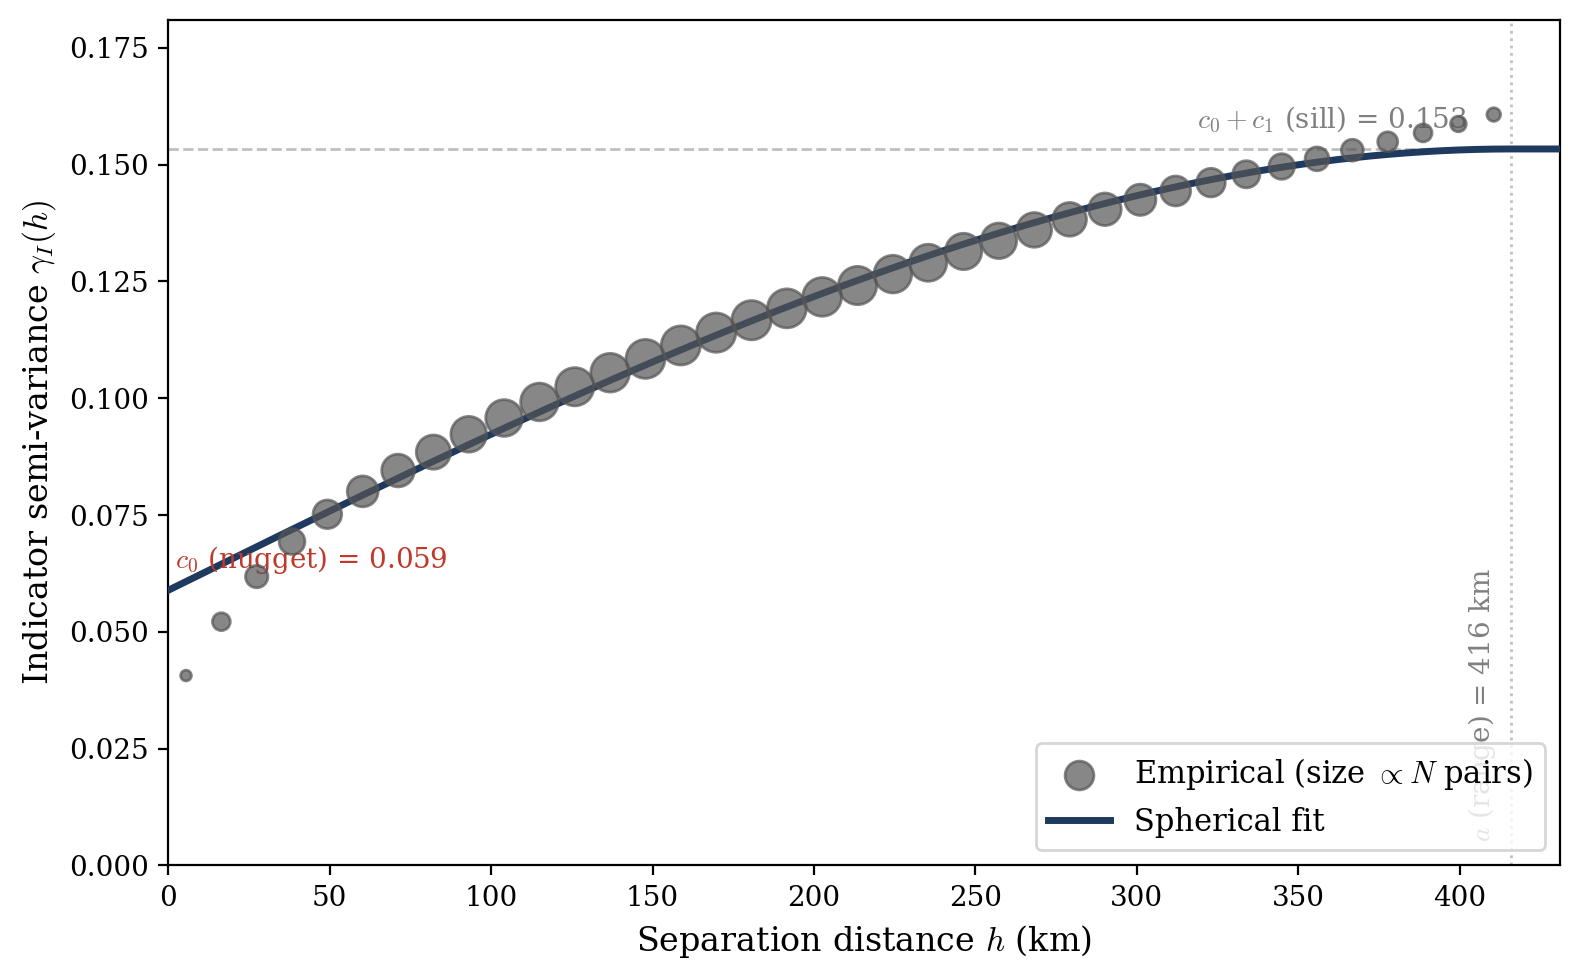
\includegraphics[width=0.85\textwidth]{images/04/indicator_variogram}
    \caption{Global indicator semi-variogram pooled across all wet days of
    the 1961--2023 record (empirical points, marker size proportional to
    the number of station pairs in each lag bin), and the fitted spherical
    model}
    \label{fig:indicator-variogram}
\end{figure}

\begin{figure}[H]
    \centering
    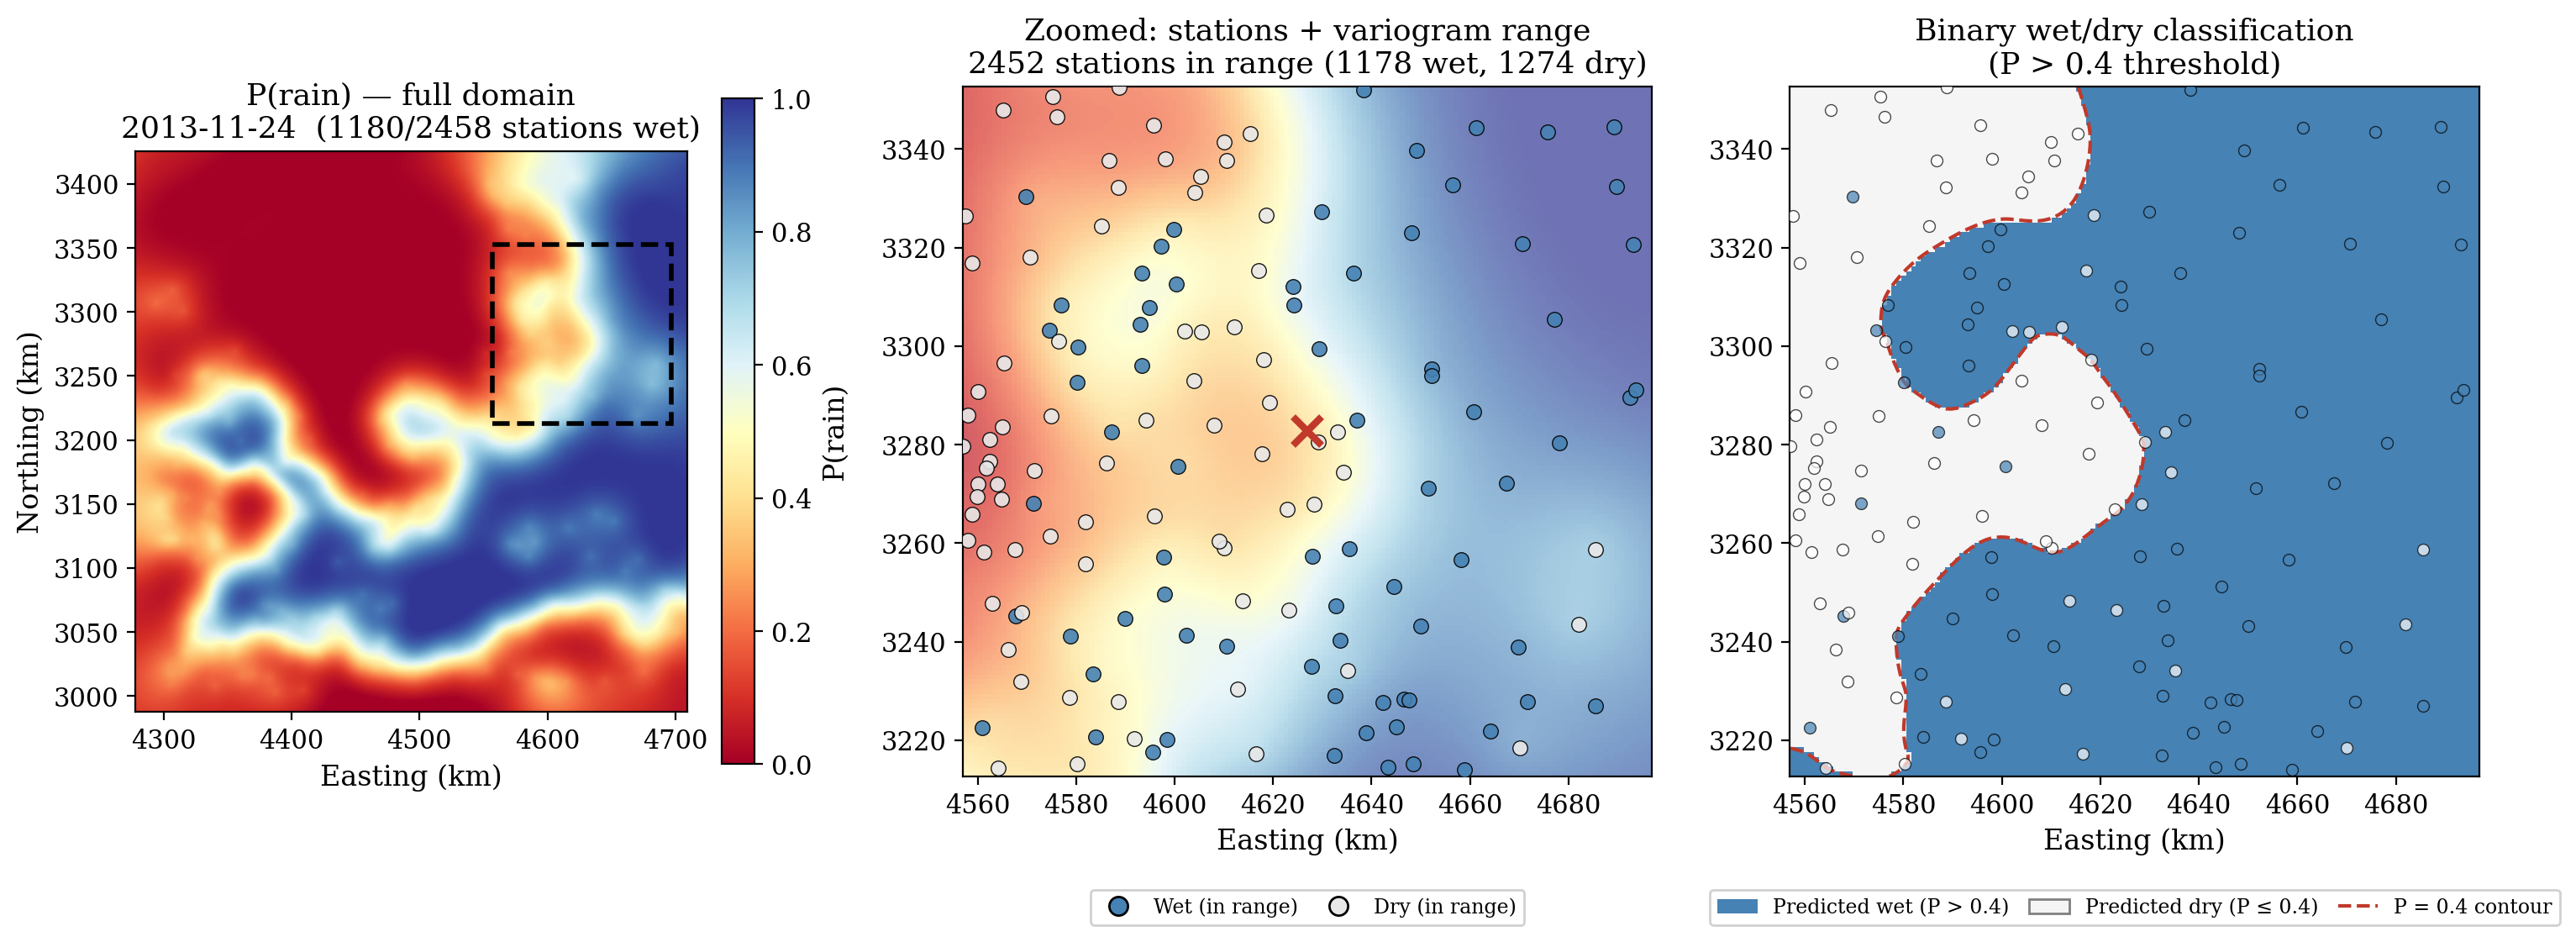
\includegraphics[width=0.95\textwidth]{images/04/indicator_kriging_2013-11-24}
    \caption{Stage~1 output for 24~November 2013 (1{,}180 wet / 1{,}258 dry
    stations). Left: interpolated rain probability $\hat{p}(\mathbf{s}_0)$
    over the full domain. Centre: zoom on the wet--dry boundary, with
    stations colour-coded by status and the indicator-variogram range
    drawn around one target cell. Right: binary classification after
    applying the $\hat{p} > 0{.}4$ threshold}
    \label{fig:indicator-kriging}
\end{figure}

%=============================================================================
\section{Stage~2: amount kriging}
\label{sec:kriging-stage2}
%=============================================================================

For cells classified as wet by Stage~1, Stage~2 estimates the precipitation
amount. It comprises three components: climatological normalisation that
removes seasonal and orographic non-stationarity
(Section~\ref{sec:detrending}), variogram fitting on the normalised values
(Section~\ref{sec:kriging-variogram}), and the kriging prediction with
Monte Carlo back-transformation to physical millimetres
(Section~\ref{sec:kriging-mechanics}).

\subsection{Climatological normalisation}
\label{sec:detrending}

Climatological normalisation (Section~\ref{sec:theory-quota}) requires
per-station monthly normals $\bar{M}(\mathbf{s}_i, m)$ as the divisor in
Equation~\eqref{eq:quota}. These are computed by double aggregation: wet-day
precipitation is summed per station, year and month, and then averaged
across all years of the record (1961--2023). This produces twelve values
per station — one per calendar month — representing the long-term seasonal
climatology at that location.

For prediction at grid cells where no station exists, the per-station
normals are extended to a continuous field by thin-plate spline (TPS)
interpolation. The TPS surface can be fitted in two dimensions on
projected coordinates $(x, y)$, capturing the large-scale spatial
gradient, or in three dimensions on $(x, y, z_{\text{elev}})$, additionally
modelling the orographic enhancement of precipitation with terrain
elevation. Both modes are computed during cross-validation; their relative
skill is compared in Section~\ref{sec:tps-experiment}.

The final precipitation prediction in millimetres is recovered by
multiplying the kriged ratio by the climatological normal at the target
cell:
\begin{equation}
  \hat{Z}(\mathbf{s}_0, t) = \hat{Q}(\mathbf{s}_0, t) \times
                              \bar{M}(\mathbf{s}_0, m(t)).
  \label{eq:back-transform}
\end{equation}

\begin{figure}[ht]
    \centering
    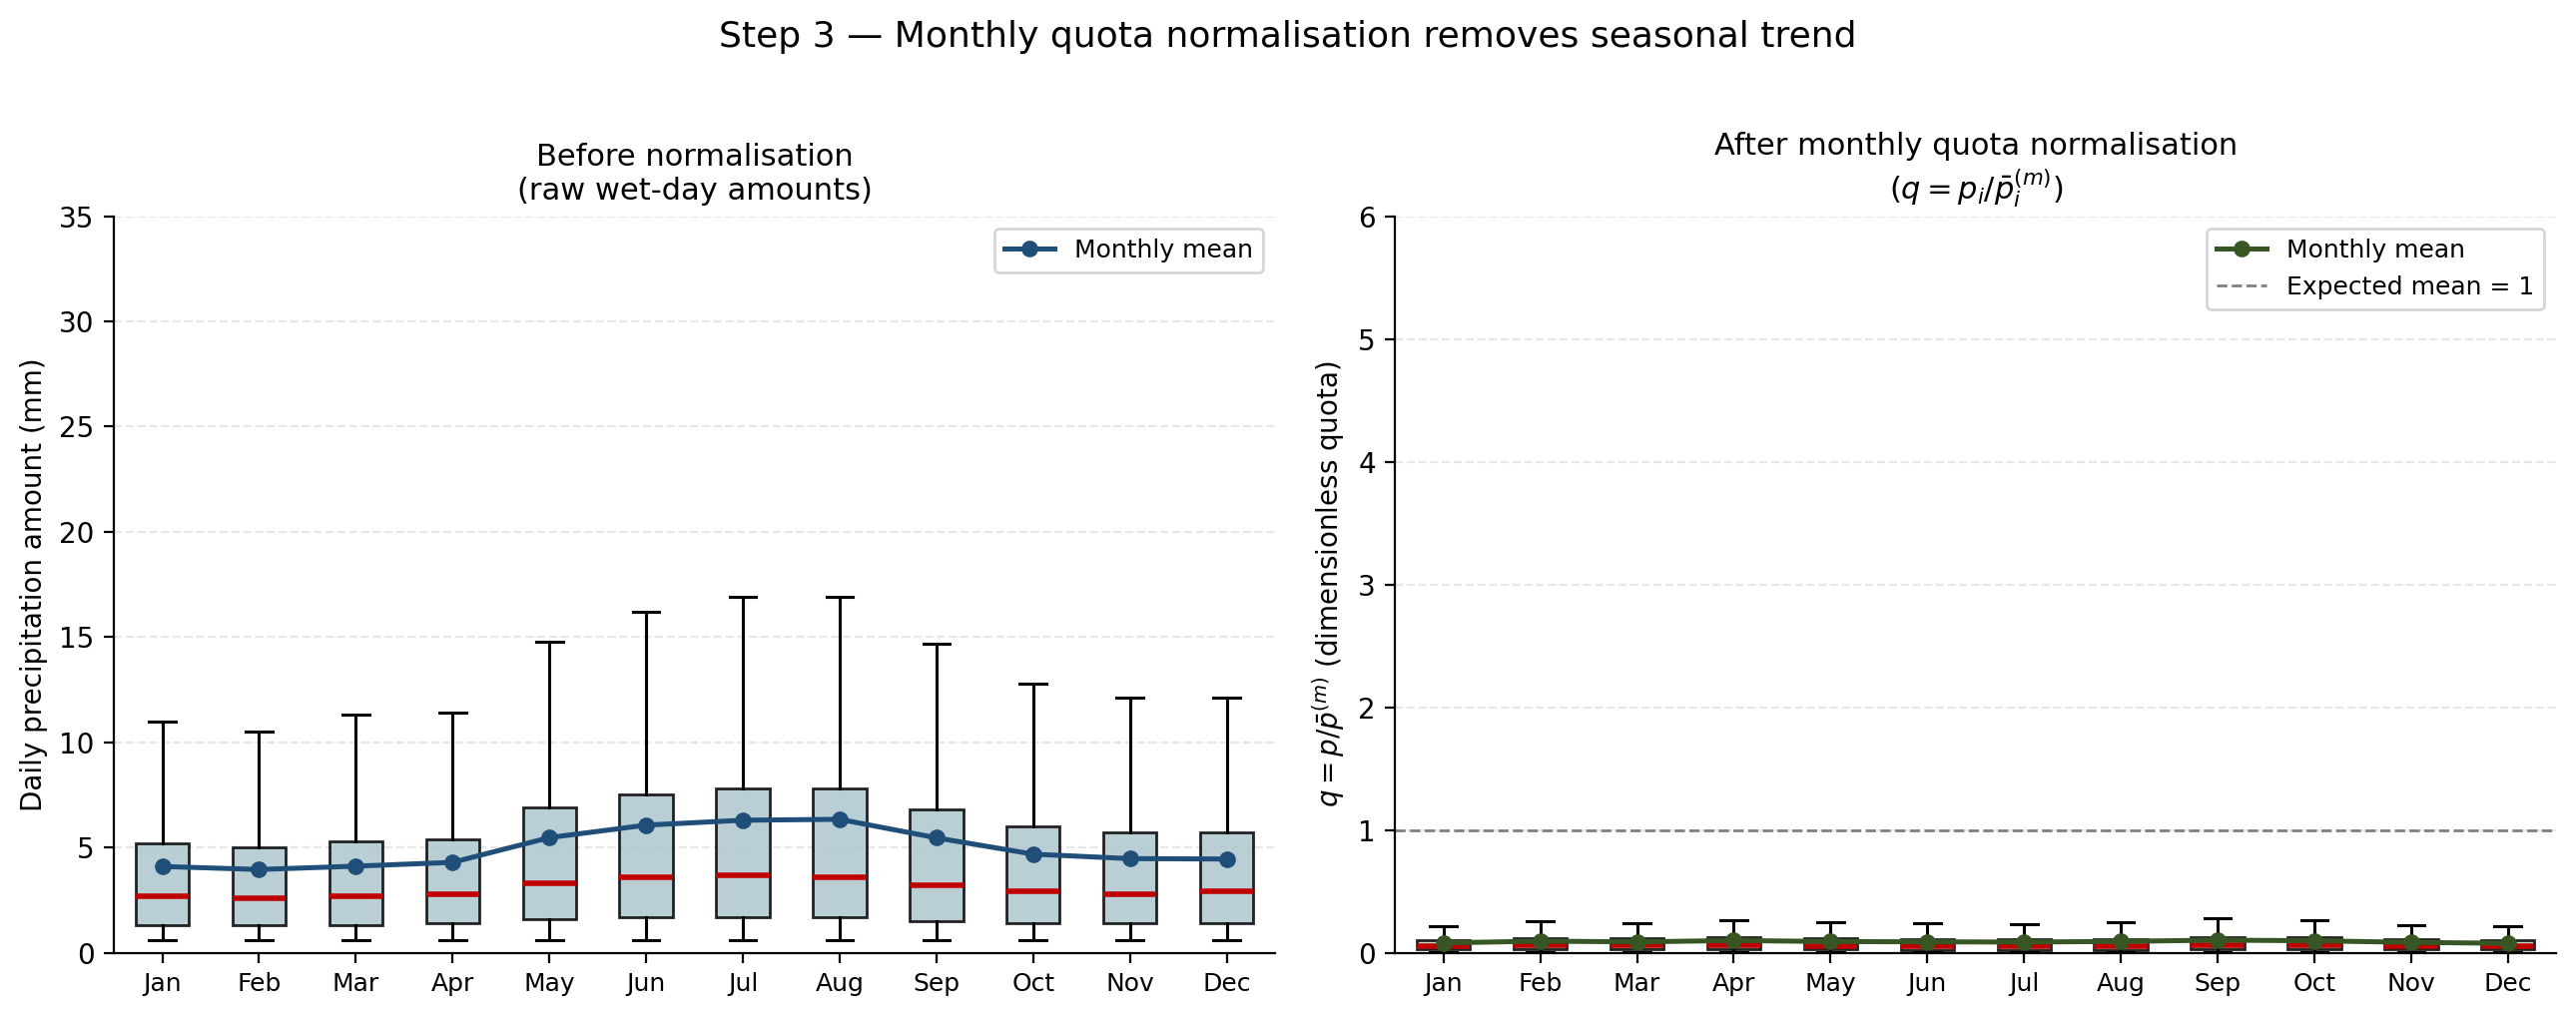
\includegraphics[width=0.95\textwidth]{images/04/prepro_seasonal}
    \caption{Monthly precipitation distributions before (left) and after
    (right) climatological normalisation. The seasonal cycle is removed
    and the distributions become approximately stationary across months}
    \label{fig:seasonal-normalisation}
\end{figure}

\subsection{Variogram fitting}
\label{sec:kriging-variogram}

Three variogram models (spherical, exponential, Gaussian) are fitted to the
pooled empirical semi-variance from all wet days of the full record
(1961--2023), following the climatological-variogram approach of
Section~\ref{sec:variogram_models} and the Marquardt weighted-least-squares
fit of Equation~\eqref{eq:marquardt-variogram}. Three transforms are tested
(none, log, normal-score), yielding nine fitted configurations in total.

\textbf{Discretisation parameters.}
The maximum lag is set to $h_{\max} = 416$~km (the 99th percentile of all
pairwise inter-station distances, Figure~\ref{fig:variogram-bins}), divided
into $N_{\text{lags}} = 38$ bins of width ${\approx}11$~km, fine enough to
resolve mesoscale structure while ensuring at least $N_{\min} = 30$ pairs per
bin \cite{cressie1993}. Under climatological pooling across all 63 years,
every bin contains several million pairs.

\begin{figure}[ht]
    \centering
    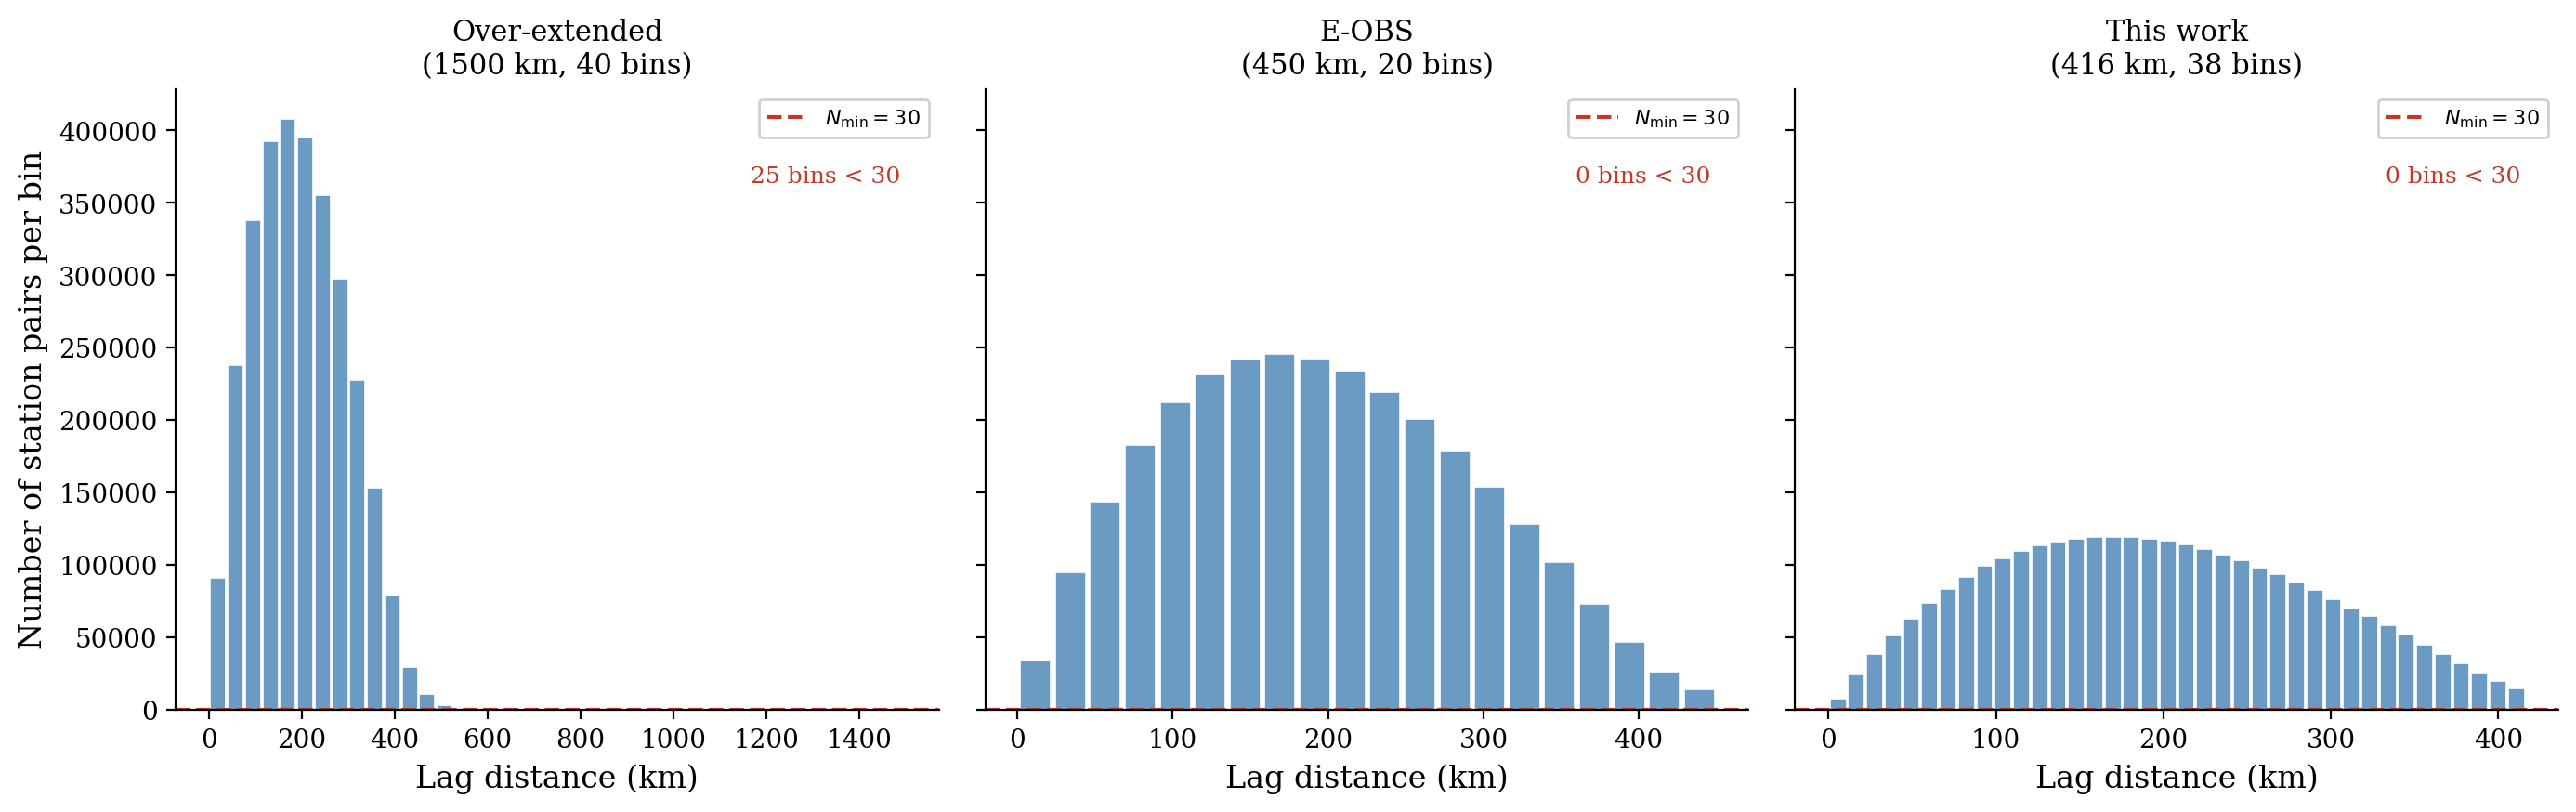
\includegraphics[width=0.95\textwidth]{images/04/variogram_bins}
    \caption{Variogram bin filling for three lag discretisations:
    over-extended (left), E-OBS settings (centre), and the settings adopted
    here (right, $h_{\max} = 416$~km, 38 bins). Red bars indicate bins with
    fewer than 30 pairs}
    \label{fig:variogram-bins}
\end{figure}

\begin{figure}[ht]
    \centering
    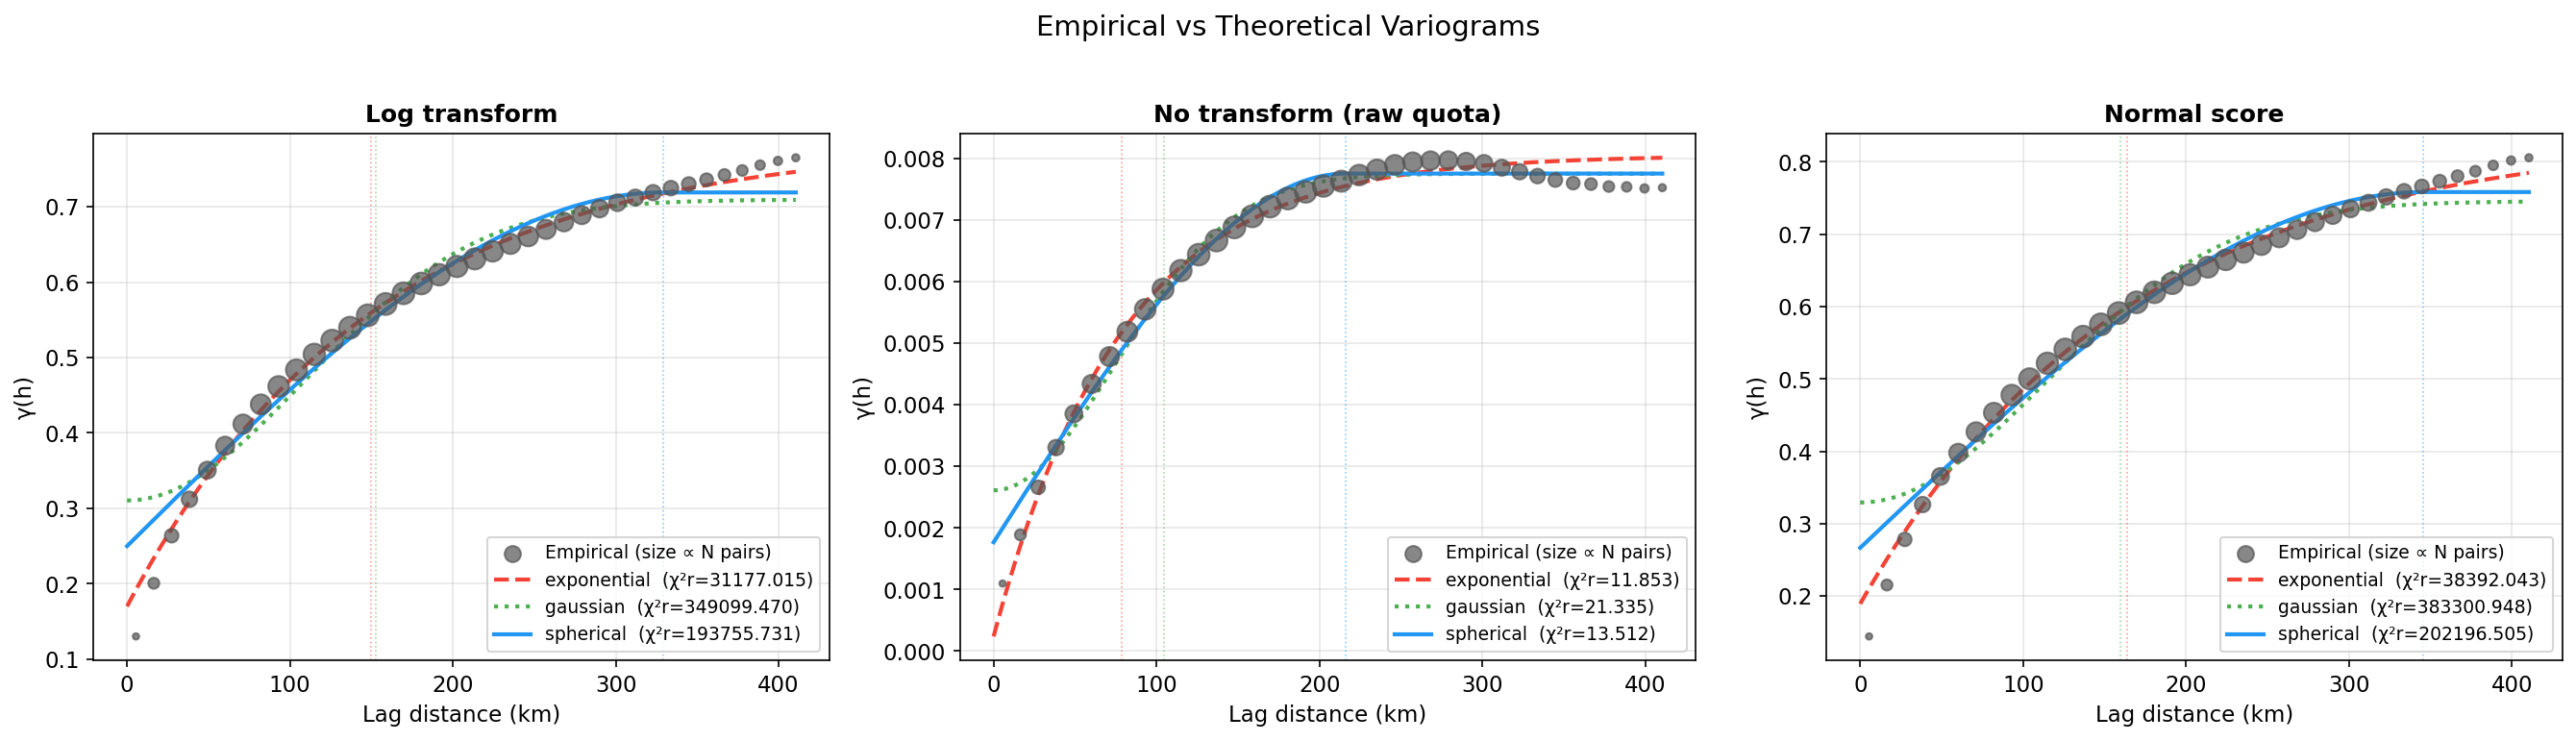
\includegraphics[width=0.95\textwidth]{images/04/variogram_fit}
    \caption{Empirical variograms with fitted models for log (left), raw
    ratio (centre), and normal-score (right) transforms. Point size is
    proportional to $N(h)$; $\chi^2_r$ is shown in the legend}
    \label{fig:variogram-fit}
\end{figure}

\begin{table}[ht]
    \centering
    \caption{Fitted variogram parameters for all nine
    (transform $\times$ model) configurations. Best $R^2$ within each
    transform is in bold.}
    \label{tab:variogram-params}
    \setlength{\tabcolsep}{4pt}
    \resizebox{\textwidth}{!}{%
    \begin{tabular}{ll ccccc}
    \toprule
    Transform & Model & Nugget $c_0$ & Sill $c_0{+}c_1$ & $a$ (km) & Eff.\ range (km) & $R^2$ \\
    \midrule
    \texttt{normal\_score} & spherical   & 0.267 & 0.754 & 342 & 342 & 0.965 \\
    \texttt{normal\_score} & exponential & 0.190 & 0.831 & 161 & 483 & \textbf{0.993} \\
    \texttt{normal\_score} & gaussian    & 0.329 & 0.742 & 158 & 273 & 0.933 \\
    \texttt{log}           & spherical   & 0.251 & 0.717 & 326 & 326 & 0.963 \\
    \texttt{log}           & exponential & 0.172 & 0.784 & 148 & 444 & \textbf{0.993} \\
    \texttt{log}           & gaussian    & 0.311 & 0.708 & 152 & 263 & 0.933 \\
    \texttt{none} (ratio)  & spherical   & 0.002 & 0.008 & 216 & 216 & 0.985 \\
    \texttt{none} (ratio)  & exponential & 0.000 & 0.008 &  79 & 236 & \textbf{0.986} \\
    \texttt{none} (ratio)  & gaussian    & 0.003 & 0.008 & 105 & 181 & 0.968 \\
    \bottomrule
    \end{tabular}%
    }
\end{table}

$R^2 = 1 - \mathrm{SS}_{\text{res}} / \mathrm{SS}_{\text{tot}}$ compares
the fitted variogram against the $N = 38$ empirical lag bins:
$\mathrm{SS}_{\text{res}}$ is the sum of squared residuals between
$\gamma_{\text{model}}(h_i)$ and $\hat{\gamma}(h_i)$, and
$\mathrm{SS}_{\text{tot}}$ is the variance of the empirical values
around their mean. Values close to $1$ indicate that the parametric
form tracks the empirical curve point-for-point; unlike $\chi^2_r$,
$R^2$ is scale-invariant and therefore directly comparable across
transforms operating in different z-spaces.

All nine configurations yield $R^2 \ge 0{.}93$, so the parametric
fits are sound and goodness-of-fit alone cannot rank them. The
selection between them is therefore decided by the cross-validated
CRPS in Section~\ref{sec:kriging-evaluation} rather than by the
variogram fit quality.

\subsection{Kriging prediction}
\label{sec:kriging-mechanics}

Given the fitted variogram, the ordinary kriging system of
Equation~\eqref{eq:kriging_system} is solved to obtain the optimal weights
$\mathbf{w}^*$ and the Lagrange multiplier $\lambda^*$, yielding the
kriging variance $\sigma^2_{\text{OK}}(\mathbf{s}_0)$ via
Equation~\eqref{eq:kriging_variance}. For brevity, $\sigma^2_K \equiv
\sigma^2_{\text{OK}}(\mathbf{s}_0)$ is used below.

A well-known property of $\sigma^2_K$ is that it depends only on station
geometry and the fitted variogram, not on the observed values
\cite{journel1989fundamentals, haylock2008european}. The Monte Carlo
back-transformation introduced below recovers intensity-dependent
uncertainty: the nonlinearity of $\varphi^{-1}$ stretches the same
$\sigma^2_K$ by different amounts depending on the rainfall intensity.

\subsubsection{Neighbourhood selection}
\label{sec:kriging-neighbourhood}

In practice, not every station participates in every grid-cell prediction.
The effective variogram range defines the distance beyond which spatial
correlation is negligible: for the spherical model it equals the range
parameter $a$ directly; for the exponential model it is $3a$ (the distance
at which $\gamma$ reaches 95\,\% of the sill); for the Gaussian model it
is approximately $\sqrt{3}\,a \approx 1.73a$.

For Stage~1 (indicator kriging), all stations within the domain participate
regardless of distance — the binary variable has a broader spatial
correlation than the precipitation amounts. For Stage~2 (amount kriging),
two restrictions are applied: only wet stations within the effective
range are considered, and when the number of wet stations exceeds a cap
of $k = 125$ only the $k$ nearest neighbours of each grid cell are kept.

\textbf{Screen effect.}
In a dense network, distant stations that lie ``behind'' closer ones
receive negative kriging weights: the information they carry is already
captured by the intervening stations, and they enter the kriging system
only as a minor trend-correction term \cite{deutsch1998gslib}. An empirical
analysis of the kriging weight distribution in this network shows that the
median number of stations carrying 90\,\% of the total positive weight is
approximately 26 (95th percentile: 34), and 99\,\% of the positive weight
is captured by a median of 51 stations. The cumulative weight curve
plateaus at 40--60 neighbours for the vast majority of days. Setting
$k = 125$ therefore preserves effectively all informative neighbours
while excluding the hundreds of distant stations that contribute only
noise through near-zero or negative weights.

\textbf{Sensitivity analysis.}
The value $k = 125$ is selected by cross-validation
(Figure~\ref{fig:sensitivity-max-wet}): CRPS is flat for $k \geq 50$, while
computation time grows steeply beyond that.

\begin{figure}[ht]
    \centering
    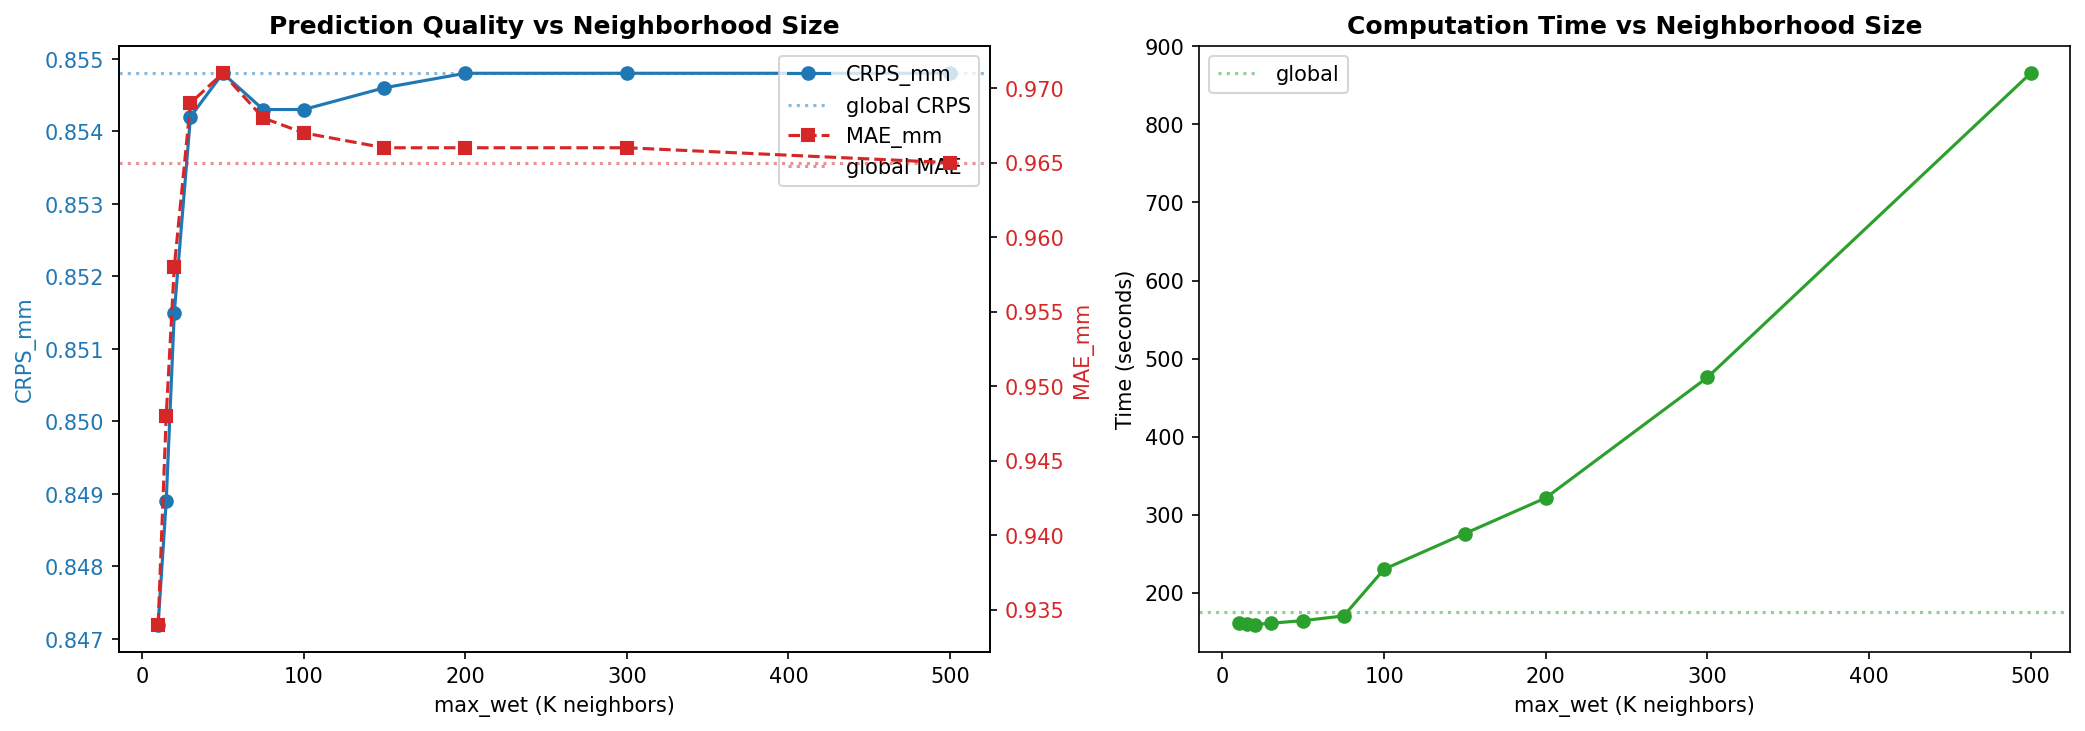
\includegraphics[width=0.95\textwidth]{images/04/sensitivity_max_wet}
    \caption{Cross-validated CRPS and computation time as a function of
    neighbourhood size $k$. Quality plateaus at $k \geq 50$; the selected
    value $k = 125$ is indicated}
    \label{fig:sensitivity-max-wet}
\end{figure}

No directional (octant or sector) search is applied. The spatial
correlation of precipitation in this domain is approximately isotropic
after climatological normalisation, so preferring stations from specific
compass directions offers no benefit over distance-based selection.

\subsubsection{Monte Carlo back-transformation}
\label{sec:kriging-mc}

The predicted ratio is obtained by drawing $K = 100$ samples from
$\mathcal{N}(\hat{z}_K, \sigma^2_K)$, back-transforming each via
$\varphi^{-1}$, and averaging \cite{journel1980lognormal}:
\begin{equation}
  \hat{Q}(\mathbf{s}_0) = \frac{1}{K}\sum_{k=1}^{K}
    \max\!\bigl(\varphi^{-1}(z^{(k)}),\, 0\bigr),
  \qquad
  \hat{Z}(\mathbf{s}_0) = \hat{Q}(\mathbf{s}_0) \times
    \bar{M}(\mathbf{s}_0, m).
  \label{eq:mc-backtrafo}
\end{equation}
The nonlinearity of $\varphi^{-1}$ produces intensity-dependent
uncertainty: variance is stretched more at high intensities than at low
ones.

%=============================================================================
\section{Cross-validation methodology}
\label{sec:kriging-cv-methodology}
%=============================================================================

For objective model selection, a \textbf{5-fold spatial cross-validation}
is used. The 2{,}458 stations are first split into 1{,}966 train and 492
holdout stations; the holdout set is never used for variogram fitting,
monthly-normal computation, or fold-internal training, and is reserved
for the cross-method evaluation of Chapter~\ref{ch:comparison}. The remaining
1{,}966 stations are partitioned into five folds via the canonical split
shared with the gradient boosting and BayesNF chapters
(\texttt{lgbm/fold\_assignment.parquet}), ensuring that all three models
are compared on identical fold assignments in Chapter~\ref{ch:comparison}.

For each fold $k$, the model is trained on the four other folds: monthly
TPS normals are refitted on the train-fold stations only, and predictions
are produced at the test-fold station coordinates. The global
climatological variogram from Section~\ref{sec:kriging-variogram} is
reused across all folds; an empirical check refits it independently on
each fold's train stations and confirms that the parameters drift by only
a few percent (variogram pooling dominates over the 20\,\% station
withdrawal because the pool aggregates ${\sim}10^{10}$ point pairs).

\textbf{Metrics.}
MAE (Equation~\eqref{eq:mae}) and CRPS (Section~\ref{sec:theory-crps}) are
the two metrics; CRPS is the primary one. For each held-out station the
$K = 100$ Monte Carlo back-transformed samples (Equation~\eqref{eq:mc-backtrafo})
form the predictive ensemble in millimetres, against which the fair CRPS
estimator (Equation~\eqref{eq:fair-crps}) is evaluated.
CRPS is computed in physical units rather than in $z$-space: different
transforms map identical physical errors to different magnitudes in
$z$-space, so evaluation in millimetres places all nine configurations
on equal footing.

%=============================================================================
\section{Cross-validation results and model selection}
\label{sec:kriging-evaluation}
%=============================================================================

Table~\ref{tab:kriging-cv} reports the cross-validation metrics for all
nine (transform $\times$ variogram) configurations, ranked by CRPS.
Metrics are computed on records on which the model predicts rainfall
($\hat{Z} \ge 0{.}4$~mm, $\approx 41\,\%$ of all records); this restricts
evaluation to the regime in which the amount stage is active.

\begin{table}[ht]
  \centering
  \caption{5-fold cross-validation results for Ordinary Kriging across all
  nine (transform $\times$ variogram) configurations (mean $\pm$ SD across
  folds). Best CRPS in bold.}
  \label{tab:kriging-cv}
  \begin{tabular}{ll cc}
    \toprule
    Transform & Variogram & MAE (mm) & CRPS (mm) \\
    \midrule
    \texttt{none} (ratio)  & exponential & $\mathbf{1.162 \pm 0.017}$ & $\mathbf{0.906 \pm 0.013}$ \\
    \texttt{normal\_score} & exponential & $1.194 \pm 0.017$ & $0.968 \pm 0.011$ \\
    \texttt{log}           & exponential & $1.203 \pm 0.017$ & $0.988 \pm 0.011$ \\
    \texttt{none} (ratio)  & spherical   & $1.347 \pm 0.017$ & $1.048 \pm 0.012$ \\
    \texttt{normal\_score} & spherical   & $1.306 \pm 0.017$ & $1.058 \pm 0.011$ \\
    \texttt{log}           & spherical   & $1.327 \pm 0.018$ & $1.093 \pm 0.011$ \\
    \texttt{normal\_score} & gaussian    & $1.579 \pm 0.016$ & $1.214 \pm 0.011$ \\
    \texttt{none} (ratio)  & gaussian    & $1.619 \pm 0.017$ & $1.219 \pm 0.012$ \\
    \texttt{log}           & gaussian    & $1.587 \pm 0.016$ & $1.245 \pm 0.011$ \\
    \bottomrule
  \end{tabular}
\end{table}

\begin{figure}[ht]
    \centering
    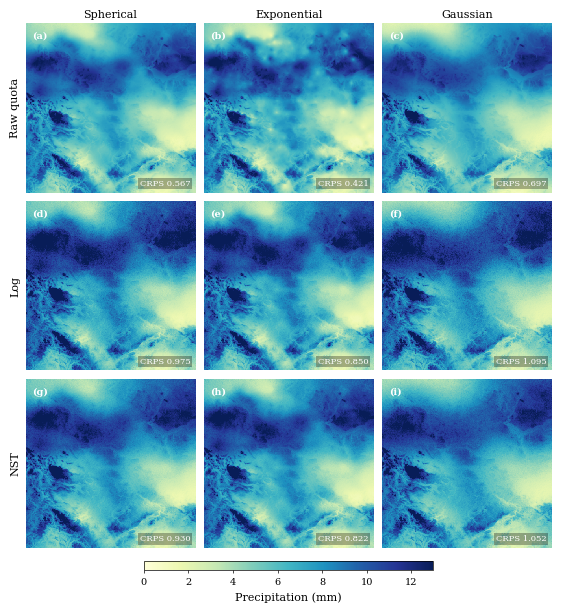
\includegraphics[width=0.95\textwidth]{images/04/predictions_all_combos}
    \caption{Spatial predictions for 1~February~2013 across all nine
    (transform $\times$ variogram) configurations}
    \label{fig:predictions-all-combos}
\end{figure}

\begin{figure}[ht]
    \centering
    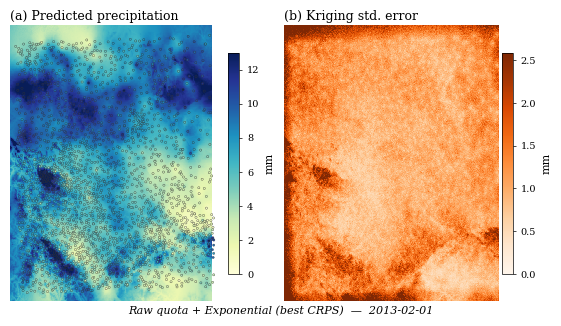
\includegraphics[width=0.95\textwidth]{images/04/best_pred_and_variance}
    \caption{Predicted precipitation (left) and kriging standard error
    (right) for the best-performing configuration (raw ratio $\times$
    exponential), 1~February~2013}
    \label{fig:best-pred-variance}
\end{figure}

\textbf{Variogram model choice.}
Haylock et al.~\cite[p.~5]{haylock2008european}, in the foundational
E-OBS methodology, tested five variogram models (Gaussian, exponential,
spherical, hole effect, power) for European precipitation kriging and
selected the model with the lowest $\chi^2$ statistic. For precipitation
amount, they found that \textit{``the modelled theoretical variograms are all
spherical, apart from precipitation amount which is exponential''}
\cite[p.~6]{haylock2008european}. The cross-validation results here
confirm this finding: for every transform, the exponential model
achieves the lowest CRPS, clearly outperforming the spherical and
Gaussian alternatives.

\textbf{Transform choice: why the raw ratio outperforms the Normal Score Transform.}
The Normal Score Transform has been recommended by Cecinati et
al.~\cite[p.~16]{cecinati2017} for kriging-based radar--gauge merging,
where it \textit{``achieves the best results overall''} among the tested
normalisation approaches. The cross-validation in this work, however,
finds that kriging on the raw climatological ratio (without any further
distributional transform) achieves a lower CRPS (0.906~mm) than the
normal-score variant (0.968~mm) or the log transform (0.988~mm).

Several factors explain this result. First, the climatological
normalisation (Section~\ref{sec:detrending}) already removes the
dominant source of non-stationarity: after detrending, the wet-day
ratios have a moderately right-skewed Gamma-like distribution, far from
the extreme skewness of raw precipitation. Second, the station network
is unusually dense (median nearest-neighbour distance of 2.1~km); in
dense networks, kriging weights are dominated by a few closest stations,
where spatial correlation is strong regardless of the distributional
shape. Third, the effective variogram range for the raw ratio
($3 \times 79 = 236$~km, exponential) is substantially shorter than for
the normal-score variant ($3 \times 161 = 483$~km), meaning the kriging
system operates with a compact, highly correlated neighbourhood instead
of mixing in weakly correlated distant stations.

Cecinati et al.~\cite{cecinati2017} evaluated the NST in the context of
Kriging with External Drift for radar--gauge merging, a setting with
additional covariates and sparser gauge networks, where enforcing
Gaussianity may provide a larger benefit. For Ordinary Kriging on
pre-detrended ratios with a dense station network, the simpler
approach without a transform suffices.

The configuration \texttt{none} $\times$ \texttt{exponential} is therefore
selected as the \textbf{final Ordinary Kriging implementation},
aligning the choice with Haylock et al.~\cite{haylock2008european} and
Hofstra et al.~\cite{hofstra2008comparison}, who use the same ratio
approach without a distributional transform for the E-OBS gridded
data set. It is the baseline against which gradient boosting
(Chapter~\ref{ch:gbm}) and Bayesian Neural Fields
(Chapter~\ref{ch:bayesnf}) are evaluated in
Chapter~\ref{ch:comparison}.

%=============================================================================
\section{Elevation contribution: 2D vs 3D TPS normals}
\label{sec:tps-experiment}
%=============================================================================

At holdout stations the station-specific monthly normal
$\bar{M}(\mathbf{s}_0, m)$ — required by the back-transformation
$\hat{Z} = \hat{Q}\,\bar{M}$
(Equation~\eqref{eq:back-transform}) — is unknown and must be interpolated
from the 1{,}966 train stations. Two TPS variants are compared: a 2D
surface fitted on projected coordinates $(x, y)$ and a 3D surface that
adds terrain elevation $(x, y, z_{\text{elev}})$. Both variants use the
same winning kriging configuration (raw ratio with the exponential
variogram) and the same 492 holdout stations; only the climatology
divisor changes.

Table~\ref{tab:tps-experiment} reports the cross-validated metrics on the
holdout set. The 3D variant reduces CRPS by 3.3\,\% and MAE by 4.2\,\%
relative to the 2D variant, confirming that elevation is an informative
covariate for the climatological field: in regions of
complex terrain, the orographic precipitation gradient cannot be captured
from planar coordinates alone, and the resulting normal estimates pass
this error through into the back-transformed amount. The 3D TPS variant
is therefore adopted as the operational climatology for the
cross-method evaluation of Chapter~\ref{ch:comparison}.

\begin{table}[ht]
  \centering
  \caption{2D vs 3D TPS monthly normals on the 492 holdout stations
  (winning combo: raw ratio $\times$ exponential), restricted to
  records on which the model predicts rainfall
  ($\hat{Z} \ge 0{.}4$~mm)}
  \label{tab:tps-experiment}
  \begin{tabular}{l cc}
    \toprule
    TPS mode & MAE (mm) & CRPS (mm) \\
    \midrule
    2D $(x, y)$              & 1.140 & 0.888 \\
    3D $(x, y, z_{\text{elev}})$ & \textbf{1.092} & \textbf{0.858} \\
    \midrule
    Relative improvement (3D over 2D) & $-4.2\%$ & $-3.3\%$ \\
    \bottomrule
  \end{tabular}
\end{table}

